% this file is called up by thesis.tex
% content in this file will be fed into the main document

%: ----------------------- introduction file header -----------------------
\chapter{Introduction}

% ----------------------- paths to graphics ------------------------

\graphicspath{{1_introduction/images/}}

% ----------------------- contents from here ------------------------
%


% \section{Context and motivation}

This thesis presents a new compression model for columnar database systems: \emph{whitebox compression}. Existing DBMSs use compression to make data smaller in terms of disk space, respectively to make queries faster by reducing I/O and memory usage and operating on the compressed data directly, without decompression. State-of-the-art columnar compression methods may not exploit all opportunities offered by the data, e.g. because these methods (RLE, FOR, DICT, DELTA) work on only one column at a time and hence cannot exploit correlations between multiple columns. Another reason is that users often use "sub-optimal" datatypes to represent their data, e.g. storing dates or numbers in strings, which are harder to compress and more expensive to operate on. Achieving high compression ratios is an important factor that influences the ability of DBMSs to scale up in terms of storage space. Compressed data leads to reducing the I/O bottleneck between disk and main memory and even between main memory and CPU if done at a granular level \cite{zukowski2006super}. Moreover, higher computation efficiency can be achieved through compression, since operating over thinner data optimizes the use of SIMD instructions.

Actual data found in real datasets tends to exhibit phenomena not found in synthetic database benchmarks like TPC-H \cite{boncz2013tpc} and TPC-DS \cite{nambiar2006making}. Not only is data often skewed in terms of value and frequency distribution, but it is also correlated across columns. Our recent efforts led to the first fully user-generated benchmark for database systems: the Public BI benchmark \cite{pbib}. Its many human-generated datasets and real data distributions open new grounds for research in the direction of columnar data compression and compressed execution. Our goal is to leverage the characteristics of these datasets for finding new methods of compression which perform well on real data rather than synthetic benchmarks. We believe the best way to achieve this is through \emph{whitebox compression}: using basic operators to create expression trees that enable efficient processing of the data.

% Existing compression methods fail to identify all compression possibilities that may exist in real data, as well as opportunities to operate directly on compressed data by pushing predicates down. We believe that, having a user-generated dataset is the perfect opportunity to learn more about real data. The goal is to find a better representation for it, which will lead to a better compression ratio and more opportunities for executing queries directly on compressed data.

% \textit{Whitebox compression} requires high performance expression evaluation provided only by modern techniques like vectorized execution or JIT code generation. These systems have so far confined themselves to the blackbox approach of only supporting a few hard-coded compression methods such as RLE, DICT, FOR and DELTA. Moreover, the problem of choosing the compression expression is workload dependent, as different data distributions and patterns can be better represented only by using dedicated combinations of operators.

% ------------ whitebox compression ------------ %

\section{Whitebox compression}

\textit{Whitebox compression} is a compression model for database systems that represents data through an expression language composed of elementary operators. Multiple operators are chained together to form an expression tree where inner nodes are operators and leaves are physical columns. A physical column is the partial representation of a logical column used for storage on disk. A logical column is the data as seen by the user. The evaluation of an expression tree on the physical columns generates the original logical columns. 

Take for example, a logical column \verb|A| which stores email addresses. It can be split by the \verb|'@'| character into 2 new columns \verb|A1| and \verb|A2|. The first one will contain the local/username part of the email address and the second one its domain (e.g. for \verb|"john.smith@gmail.com"| \verb|A1| will store \verb|"john.smith"| and \verb|A2| will store \verb|"@gmail.com"|). The second column will then be compressed with dictionary encoding to exploit the small number of unique email address domains. Stored together, email addresses are not compressible because of the uniqueness of the usernames. Through \textit{whitebox} representation, subparts of the data can be compressed independently.

\begin{figure}[h]
  \centering
  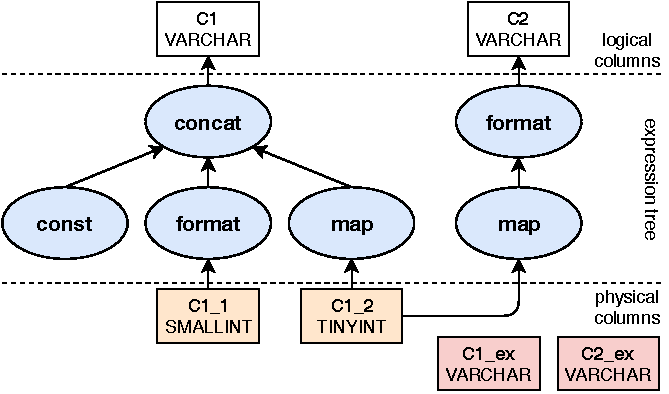
\includegraphics[width=0.75\linewidth]{intro-example_1.pdf}
  \caption{Whitebox representation example}
  \label{fig:intro:whitebox:example}
\end{figure}

Figure~\ref{fig:intro:whitebox:example} illustrates the general concept of \textit{whitebox compression}. \verb|C1| and \verb|C2| are 2 logical columns represented through elementary operator expressions as functions of the physical columns \verb|C1_1| and \verb|C1_2|. The operators are, in this example: \verb|concat|, \verb|format|, \verb|map| and \verb|const|. Chained together, they form \textit{expression trees} that transparently describe the columnar transformations applied to the data. Values that do not match the expressions are stored in the exception columns \verb|C1_ex| and \verb|C2_ex|.

\textit{Whitebox} representation creates compression opportunities. While in the original format, columns cannot be compressed through existing lightweight techniques, the physical columns resulting after applying the operator expressions are storing data more compactly. E.g. string columns are decomposed into subcolumns based on the different distributions of substring components and redundancy is eliminated by representing correlated columns as functions of the same physical columns. This process leads to efficient representation of the data in columns with appropriate datatypes and sparse exception columns.

% TODO: different example here.
% Another example is the logical column "customer\_id" with values of the following format: "customer\_no\_\$\{x\}", where \$\{x\} is a fixed length 6 digit integer (e.g. "customer\_no\_000001", "customer\_no\_000736", etc.). We can represent this column through the expression: \emph{format("customer\_no\_\%06d", delta\_inv(\$\{x\}))}. Here we have the \emph{format} operator which takes as parameter a format string similar to the \emph{printf} function in C. The second operator is \emph{delta\_inv}, meaning the decompression function for DELTA. The corresponding compression tree is depicted in Figure \ref{fig:intro:whitebox:example}.

% In both examples the data is transformed in a way that creates compression opportunities. While in the original format the data cannot be compressed through lightweight techniques, the columns resulting after applying the operators are either reduced to a single value ("customer\_no\_") or compressed with DELTA or DICT.

The difference between \textit{blackbox compression} and \textit{whitebox compression} is best perceived from the system's perspective. Table~\ref{tab:intro:blackboxwhitebox} shows a comparison between the 2 models.

\begin{table}[h]
\centering
\makebox[\textwidth][c]{
\begin{tabular}{l|l|l}
                    & \multicolumn{1}{c|}{Blackbox} & \multicolumn{1}{c}{Whitebox}          \\ \hline
Nature              & hardcoded, opaque             & generic, flexible, transparent        \\
Header info & identifier (e.g. PFOR)        & operator expression, self-descriptive \\
Output              & block of data                 & columns (allows recursion)            \\
Exceptions          & included in the data block    & separate columns                     
\end{tabular}
}
\caption{Blackbox vs. whitebox comparison}
\label{tab:intro:blackboxwhitebox}
\end{table}

A \textit{blackbox compression} system takes as input a column and outputs a block of data, containing both the compressed values and the exceptions, stored in a format only known by the system. In contrast, a \textit{whitebox compression} system takes as input a set of columns and outputs an expression tree and other columns. The representation of the columns is transparent and self-descriptive, which enables  partial decompression of the data by pushing operators down the compression tree at query execution time. The \textit{whitebox compression} model is generic and flexible, allowing recursive compression of columns---including exceptions. It can be easily extended with new operators and adapted according to the system's needs and data characteristics.

\iffalse
- distinction between whitebox and blackbox compression/representation
- see presentation slides
\fi

% ------------ research questions ------------ %

% \newpage
\section{Research questions}

The goal of our project is to explore the concept of \emph{whitebox compression} with the purpose of finding a better way to compress human-generated data. To this end, we defined a list of scientific questions that we answer during our research.
\begin{enumerate}[1)]
    \item What does real user generated data look like---specifically in the case of the Public BI benchmark?
    \begin{enumerate}[a)]
        \item What patterns can we find in the columns of each dataset?
        \item Inefficient ways of representing data?
        \item "Wrong" type used to define data (e.g. number stored as string, etc.)?
    \end{enumerate}
    \item How good are existing compression schemes at compressing real data?
    \begin{enumerate}[a)]
        \item Do they make the most out of the properties of the data?
        \item Is there room for improvement?
    \end{enumerate}
    \item Can we represent the logical columns more compactly through an expression tree composed of elementary operators?
    \begin{enumerate}[a)]
        \item What kind of operators are suitable for expressing the data and transforming it to physical columns?
        \item What will the compression ratio be?
        \item Can we exploit correlations between multiple logical columns by sharing the physical columns in their expressions?
    \end{enumerate}
    \item Can we create an automatic learning process that will generate suitable compression trees for each column?
    \begin{enumerate}[a)]
        \item Will it provide a high compression ratio?
        \item How will it compare to existing solutions?
    \end{enumerate}
\end{enumerate}

The focus of this thesis is on learning patterns from the data and automatically generating expression trees for more compact data representation---everything optimized for size. An additional, but equally important aspect of this topic is query execution time and whether it can be improved through \textit{whitebox compression}. We leave this subject for future work. We defined the corresponding research question below for completeness, but we do not answer it in this thesis. 
\begin{enumerate}[1)]
    \setcounter{enumi}{4}
    \item Can we achieve compressed execution with the \textit{whitebox compression} model?
    \begin{enumerate}[a)]
        \item Can we exploit SIMD in the scan?
        \item Will there be lazy decompression opportunities?
        \item Can we push query predicates down the compression tree?
    \end{enumerate}
\end{enumerate}

We carried out our research and structured this thesis according to these questions. We present related work in Chapter~\ref{ch:relatedwork}. We performed a characterisation of the Public BI benchmark and then manually analyzed its datasets in search for patterns and compression opportunities not exploited by the existing systems (Chapter~\ref{ch:pbib}). Based on our findings, we defined the \textit{whitebox compression} model, the expression language and all its characteristics in Chapter~\ref{ch:exprlang}. Furthermore, we defined algorithms that automatically detect compression opportunities and generate compression trees that represent data more compactly (Chapter~\ref{ch:automaticlearning}). Finally, we evaluate our proof-of-concept implementation of \textit{whitebox compression} against an existing database system and an estimator model baseline (Chapter~\ref{ch:evaluation}).
